
%
%
%
The hybridized SBP-SAT formulation discretizes this problem into the form 

%
%
%
\begin{equation}
    \left[\begin{array}{cc}
        \textbf{M}             & \textbf{F} \\
        \textbf{F}^{\intercal} & \textbf{D}
    \end{array}\right] 
    \left(\begin{array}{c}
        \textbf{u} \\
        \symbf{\lambda}
    \end{array}\right) = 
    \left(\begin{array}{l}
        \bar{\textbf{g}} \\
        \gbd
    \end{array}\right),
    \label{eqn:hybrid_system}
\end{equation}

%
%
%
\noindent
From the Schur complement we have $(\textbf{D} - \textbf{F}^{\intercal} \textbf{M}^{-1} \textbf{F}) \symbf{\lambda} = \gbd - \textbf{F}^{\intercal} \textbf{M}^{-1} \bar{\textbf{g}}$. 
This is solved in two parts: the global problem,

%
%
%
\begin{subequations}
\begin{equation}
\symbf{\lambda}_{\textbf{A}} \coloneqq \gbd - \textbf{F}^{\intercal} \text{solve}(\textbf{M}, \bar{\textbf{g}}),
\label{eqn:global_system_a}
\end{equation}
\begin{equation}
\symbf{\lambda}_{\textbf{b}} \coloneqq \textbf{D} - \textbf{F}^{\intercal} \text{solve}(\textbf{M}, \textbf{F}),
\label{eqn:global_system_b}
\end{equation}
\begin{equation}
\symbf{\lambda} \coloneqq \text{solve}(\symbf{\lambda}_{\textbf{A}}, \symbf{\lambda}_{\textbf{b}}),
\label{eqn:global_system_c}
\end{equation}
\end{subequations}
\noindent
and the local problem,
\begin{equation} 
\textbf{u} \coloneqq \text{solve}(\textbf{M}, (\bar{\textbf{g}} - \textbf{F} \times \symbf{\lambda})).
\label{eqn:local_system}
\end{equation}

%
%
%
\noindent
In this scheme, multiple elements with continuous domains are coupled with boundary coefficients resembling Dirichlet boundary conditions. 
The boundary coefficients are factored out to $\textbf{F}$ and $\textbf{F}^{\intercal}$, leaving $\textbf{M}$ with a block diagonal non-zero pattern. 

%
%
%
\begin{figure}
	\centering
	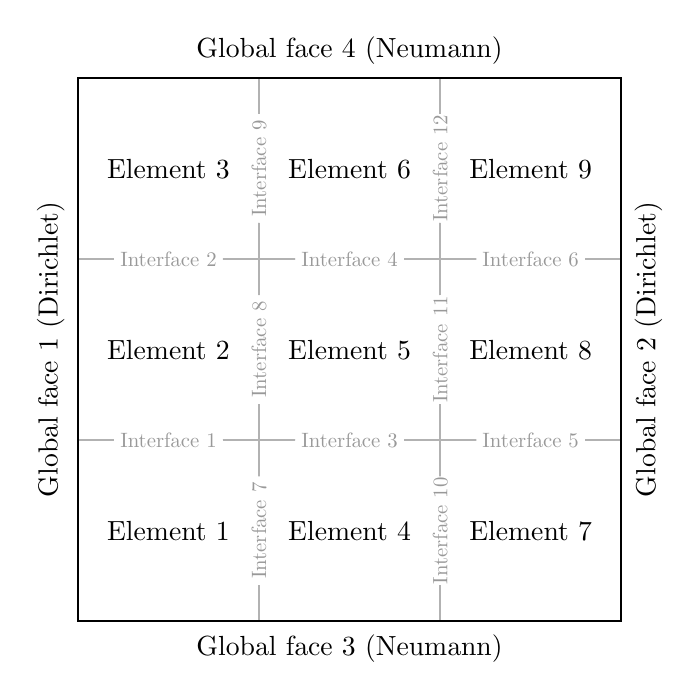
\begin{tikzpicture}[scale=2.3]
\draw[step=1cm,black!30,line width=0.3mm] (0, 0) grid (3, 3);
\draw[line width=0.3mm] (0, 0) rectangle (3, 3);

\fill[white] (0.5cm, 1cm) circle (0.3cm);
\node[color=black!40, scale=0.75] at (0.5cm, 1cm) {Interface 1};
\fill[white] (0.5cm, 2cm) circle (0.3cm);
\node[color=black!40, scale=0.75] at (0.5cm, 2cm) {Interface 2};
\fill[white] (1.5cm, 1cm) circle (0.3cm);
\node[color=black!40, scale=0.75] at (1.5cm, 1cm) {Interface 3};
\fill[white] (1.5cm, 2cm) circle (0.3cm);
\node[color=black!40, scale=0.75] at (1.5cm, 2cm) {Interface 4};
\fill[white] (2.5cm, 1cm) circle (0.3cm);
\node[color=black!40, scale=0.75] at (2.5cm, 1cm) {Interface 5};
\fill[white] (2.5cm, 2cm) circle (0.3cm);
\node[color=black!40, scale=0.75] at (2.5cm, 2cm) {Interface 6};

\fill[white](1cm, 0.5cm) circle (0.3cm);
\node[color=black!40, rotate=90, scale=0.75] at (1cm, 0.5cm) {Interface 7};
\fill[white] (1cm, 1.5cm) circle (0.3cm);
\node[color=black!40, rotate=90, scale=0.75] at (1cm, 1.5cm) {Interface 8};
\fill[white] (1cm, 2.5cm) circle (0.3cm);
\node[color=black!40, rotate=90, scale=0.75] at (1cm, 2.5cm) {Interface 9};
\fill[white] (2cm, 0.5cm) circle (0.3cm);
\node[color=black!40, rotate=90, scale=0.75] at (2cm, 0.5cm) {Interface 10};
\fill[white] (2cm, 1.5cm) circle (0.3cm);
\node[color=black!40, rotate=90, scale=0.75] at(2cm, 1.5cm) {Interface 11};
\fill[white] (2cm, 2.5cm) circle (0.3cm);
\node[color=black!40, rotate=90, scale=0.75] at (2cm, 2.5cm) {Interface 12};


\draw (0.5cm, 0.5cm) -- (0.5cm, 0.5cm) node[anchor=center] {Element 1};
\draw (0.5cm, 1.5cm) -- (0.5cm, 1.5cm) node[anchor=center] {Element 2};
\draw (0.5cm, 2.5cm) -- (0.5cm, 2.5cm) node[anchor=center] {Element 3};
\draw (1.5cm, 0.5cm) -- (1.5cm, 0.5cm) node[anchor=center] {Element 4};
\draw (1.5cm, 1.5cm) -- (1.5cm, 1.5cm) node[anchor=center] {Element 5};
\draw (1.5cm, 2.5cm) -- (1.5cm, 2.5cm) node[anchor=center] {Element 6};
\draw (2.5cm, 0.5cm) -- (2.5cm, 0.5cm) node[anchor=center] {Element 7};
\draw (2.5cm, 1.5cm) -- (2.5cm, 1.5cm) node[anchor=center] {Element 8};
\draw (2.5cm, 2.5cm) -- (2.5cm, 2.5cm) node[anchor=center] {Element 9};


\node[rotate=90] at (-0.15cm, 1.5cm) {Global face 1 (Dirichlet)};
\node[rotate=90] at (3.15cm, 1.5cm) {Global face 2 (Dirichlet)};
\node at (1.5cm, -0.15cm) {Global face 3 (Neumann)};
\node at (1.5cm, 3.15cm)  {Global face 4 (Neumann)};
\end{tikzpicture}
	\caption{An illustration the volume, and arrangement of interfaces described by a 3-by-3 instance of the hybrid problem specified in \eqref{eqn:hybrid_system}.}
	\label{fig:volume_diagram}
\end{figure}

%
%
%
\noindent
This permits us \textbf{a)} to compute much larger problems with less memory, especially if the problem is largely homogeneous, and \textbf{b)} to reduce the computational complexity of solving the system by instead solving several smaller systems. 
In both cases this allows us express the equations (\ref{eqn:global_system_a}--\ref{eqn:global_system_c}, \ref{eqn:local_system}) as a concatenation of smaller problems. 

%
%
%
To form the smaller problems we decompose the sub-matrices $\textbf{M}$, $\textbf{F}$, $\textbf{F}^{\intercal}$, and $\textbf{D}$. 
For example, as $\textbf{M}$ is block-diagonal, we store each non-zero component in $\textbf{M}$ as a matrix. 
For homogeneous problems several of the non-zero components in $\textbf{M}$ are identical, requiring only one copy for each unique component for a given shared-memory context.
A similar structure exists for $\textbf{F}$ and $\textbf{F}^{\intercal}$, though the homogeneity of these matrices depends on the mesh structure, not the domain structure. \\

%
%
%
\begin{aside}
    For this work we consider a specialization of the problem where both the mesh and each element are square. 
    Here, the total number of elements, $\ell^2$, is the square of the number of elements on any face of the \emph{global} domain, $\ell$. 
    Additionally, each the number of volume points in each element, $n^2$, is the square of the number of volume points along any face $n$. 
    Finally, there are only 4 unique interfaces, 1 for each interior face of an element.
\end{aside}

%
%
%
\noindent
In a 3-by-3 example of the problem we reconstruct $\textbf{F}$ from the representational matrix, $\textbf{F}^{\text{ind}}$, and the set of unique $\textbf{F}^{i}$ sub-matrices, substituting the appropriate sub-matrix in place of the integer value, \emph{i.e.},

\begin{subequations}
\begin{equation}
	\textbf{F} = \textbf{F}^{\text{ind}}\left[i/\textbf{F}^{i}\right] \text{ where } i \neq 0,
    \label{eqn:finc}
\end{equation}
\begin{equation}
	{\footnotesize
    \begin{array}{c}
        {\color{gray} \hspace{-1em} \textit{Interface index}} \\
        {\color{gray}
        \begin{array}{C{0.25em}C{0.5em}C{0.5em}C{0.5em}C{0.5em}C{0.5em}C{0.5em}C{0.5em}C{0.5em}C{0.5em}C{0.5em}C{0.5em}C{0.5em}C{0.5em}}
        {}&{1}&{2}&{3}&{4}&{5}&{6}&{7}&{8}&{9}&{10}&{11}&{12}&{}\\
        \end{array}} \\
        \textbf{F}^{\text{ind}} = \left[\begin{array}{cccccccccccc}
         4 &{·}&{·}&{·}&{·}&{·}& 2 &{·}&{·}&{·}&{·}&{·}\\
         3 & 4 &{·}&{·}&{·}&{·}&{·}& 1 &{·}&{·}&{·}&{·}\\
        {·}& 3 &{·}&{·}&{·}&{·}&{·}&{·}& 2 &{·}&{·}&{·}\\
        {·}&{·}& 4 &{·}&{·}&{·}& 1 &{·}&{·}& 2 &{·}&{·}\\
        {·}&{·}& 3 & 4 &{·}&{·}&{·}& 1 &{·}&{·}& 2 &{·}\\
        {·}&{·}&{·}& 3 &{·}&{·}&{·}&{·}& 1 &{·}&{·}& 2 \\
        {·}&{·}&{·}&{·}& 4 &{·}&{·}&{·}&{·}& 1 &{·}&{·}\\
        {·}&{·}&{·}&{·}& 3 & 4 &{·}&{·}&{·}&{·}& 1 &{·}\\
        {·}&{·}&{·}&{·}&{·}& 3 &{·}&{·}&{·}&{·}&{·}& 1 \\
        
        \end{array}\right] {\color{gray}
        \begin{array}{C{1em}}
        1 \\ 2 \\ 3 \\ 4 \\ 5 \\ 6 \\ 7 \\ 8 \\ 9
        \end{array}{\rotatebox[origin=c]{90}{\textit{Element index}}}} \\
    \end{array}}
    \label{eqn:find}
\end{equation}
\begin{equation}
	\left\{\textbf{F}^{1},\textbf{F}^{2},\textbf{F}^{3},\textbf{F}^{4}
	\right\}.
    \label{eqn:fine}
\end{equation}
\end{subequations}

\noindent
In this problem there are only 4 unique sub-matrices because the mesh of elements consists of identically sized 4-sided elements. 
The location of entries in each row of \eqnref{eqn:find} correspond to the orientation of interfaces along a given element seen in \figref{fig:volume_diagram}, \emph{e.g.}, element 2 has interfaces 1, 2, and 8, corresponding to non-zeros in the identical columns in row 2 of $\textbf{F}^{\text{ind}}$.

